% ----------------------------------------------------
% Methodology
% ----------------------------------------------------

\chapter{Methodology}\label{ch:methodology}

\section{Device Design}

\subsection{Salinity Measurement Method}

\textit{help}
Of the available methods for measuring salinity, the most common method used in oceanography is the conductivity method.
This is because conductivity of salt water is the easiest to repeatably measure and provides the most consistent accuracy.
Information on other methods can be found in the literature review.

One of the most common methods of measuring conductivity of a liquid is to measure the resistance between two electrodes or probes in the liquid and use that to determine its conductivity.
The shape and material of the probes are an important factor which affect the measurement accuracy and drift as well as the ease of calculation from resistance to conductivity.

\subsection{Conductivity Probe Material}

Ideal probes for measuring conductivity in salt water need to have zero resistance, infinite corrosion resistance and be able to confine the electrical current in the water to a specific volume.
The zero resistance will allow the resistance that it measured to be entirely due to the water, although most conductive materials have a conductivity in the order of $10^8 S/m$ which causes negligible resistance compared to water which has a conductivity range of $0-5 S/m$. %https://atlas-scientific.com/blog/water-conductivity-range/ https://byjus.com/physics/conductivity-of-water/#:~:text=Viscosity%20And%20Density-,Salt%20Water%20Conductivity,and%20chlorine%20ions%20(NaCl).
The infinite corrosion resistance will allow the probes to last indefinitely in the highly corrosive salt water.
The confinement of the electrical current allows for an easier calculation of the conductivity $\rho$ from resistance $R$ if the cross-sectional area $A$ and length $l$ of the water between the probes is known as shown by \refeqn{eqn:conductivity-from-resistance}.
\begin{equation}
    \rho = \lfrac{RA}{l}
    \label{eqn:conductivity-from-resistance}
\end{equation}
There are several metals known for their corrosion resistance which are used in corrosive environments including marine environments.
The most abundant of these are aluminium and stainless steel, followed by nickel and copper alloys, such as Monel or brass, and finally titanium.
Additionally, the precious metals gold, silver and platinum are also known for their exceptional corrosion resistance which exceeds the aforementioned metals, although they are significantly more expensive.

The choice of material aimed at using materials with the highest corrosion resistance while still choosing materials that were attainable and within this project's budget.
Titanium is the most corrosive resistant of the non-precious metals and has an acceptable resistivity of $4.5\e{-7}\Omega\cdot m$ which is about 25 times that of copper.
Titanium wire was available through off-cuts from a project being conducted by the Chemical Engineering Department of the University of Cape Town, and thus it was possible to use this material for the electrodes.

Of the precious metals, gold is one of the most accessible as it is a common material used in \glspl{pcb} manufacturing primarily because of its high corrosion resistance while it maintains a low resistivity of $2.44\e{-8}\Omega\cdot m$ similar to copper.
\gls{enig} \gls{pcb} manufacturing is a process where nickel followed by gold are deposited onto the copper of the \gls{pcb} using chemical reactions.
While this process is expensive, it is affordable within this project's budget and made gold a possible material for the electrodes.

Gold and titanium were both used as electrodes for this project due to their high corrosion resistance, conductivity and availability.

\subsection{Conductivity Probe Design}

Gold electrodes made using the \gls{enig} \gls{pcb} manufacturing process were chosen to be the primary electrodes for the device.
The high corrosion resistance and conductivity of gold were advantageous, and the \gls{pcb} allowed the probes to be made with a known area and length of the water between the probes.

Some scientific papers that attempt to measure salinity have an uncertainty on whether salt water has a constant resistivity relative to the voltage applied to it or not.
In order to verify this, the resistance of the water between the probes needed to be measured at different voltages while other factors were kept constant which necessitated close attention to the fringing effect of the electrical current between the probes.
Thus, wide flat pads were used on the \gls{pcb} probes, and they were placed them close together to reduce the amount of current fringing allowing for a more accurate calculation of the conductivity.
To further reduce the fringing, a fringe guard was added to the probes which consisted of a pad that outlined the main conductivity pads that repeated the same voltage as the main pads using an op-amp which would allow for the fringing to be taken up by the fringe guard and not affect the resistance measurement.

The dimensions of the gold electrodes were chosen somewhat arbitrarily with the pads having a large area while being placed relatively close together to reduce the fringing but not too close to prevent water from flowing between the pads.
Additionally, the aim was to keep the resistance between the pads low to lower the amount of voltage required to generate a current through the water thus further reducing the fringing. 
The gold electrodes were designed with a $20mm \times 20mm$ pad area with a $2mm$ wide fringe guard surrounding the majority of the pad and were spaced $10mm$ apart as shown in \reffig{fig:gold-electrode}.
This gave a resistance of $3.75\Omega$ to $6.25\Omega$ between the gold electrodes for salinities of $40$ to $25$ on the practical salinity scale respectively.
\begin{figure}
    \centering
    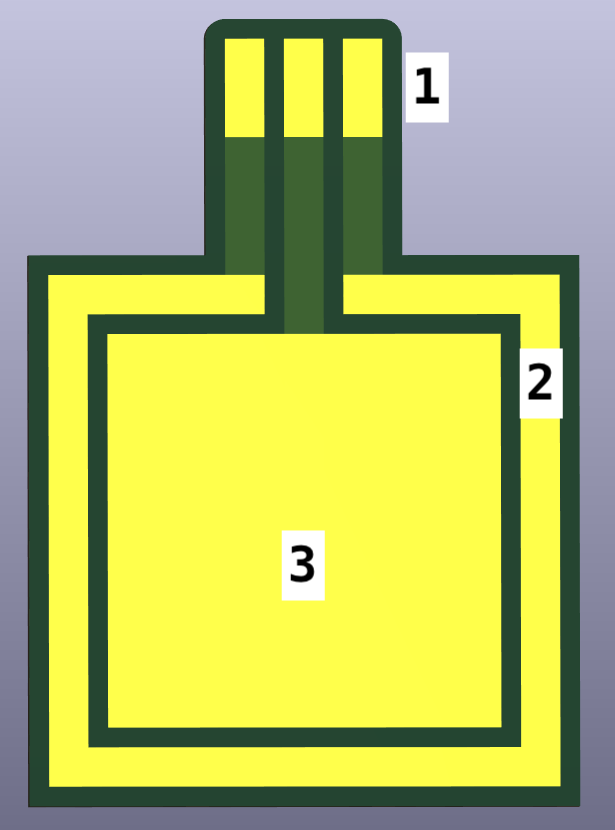
\includegraphics[width=0.5\textwidth]{Figures/GoldElectrode}
    \caption{The gold electrode \gls{pcb} design.}
    \label{fig:gold-electrode} %chktex 24
\end{figure}

The titanium electrodes are substantially simpler and cheaper than the gold electrodes and would be the preferred electrodes if the fringing effect could be accounted for.
Provided the testing with the gold electrodes is able to prove a constant resistance-voltage relationship, the fringing effect between the titanium electrodes could be measured and accounted for allowing for them to be used as the primary electrodes in a future iteration of the device.
The titanium wire that was available for this project was $1mm$ in diameter and in order to account for the unknown resistance between the electrodes, the design allowed for an adjustable spacing between the electrodes and adjustable electrode length.

\subsection{Resistance Measurement Method}

The most common and practical method of measuring resistance is to use a resistor divider circuit.
Current meters are also used to measure resistance, but most of them use the same principle of a resistor divider circuit to determine the current.
This project chose to use a large $R_1$ in series with the electrodes such that the voltage between the probes would be lower which would further reduce the fringing effect.
The measurement taken from the voltage divider was then amplified by a factor of 11 to increase the resolution of the measurement.

\subsection{Circuit Overview}

\begin{figure}
    \centering
    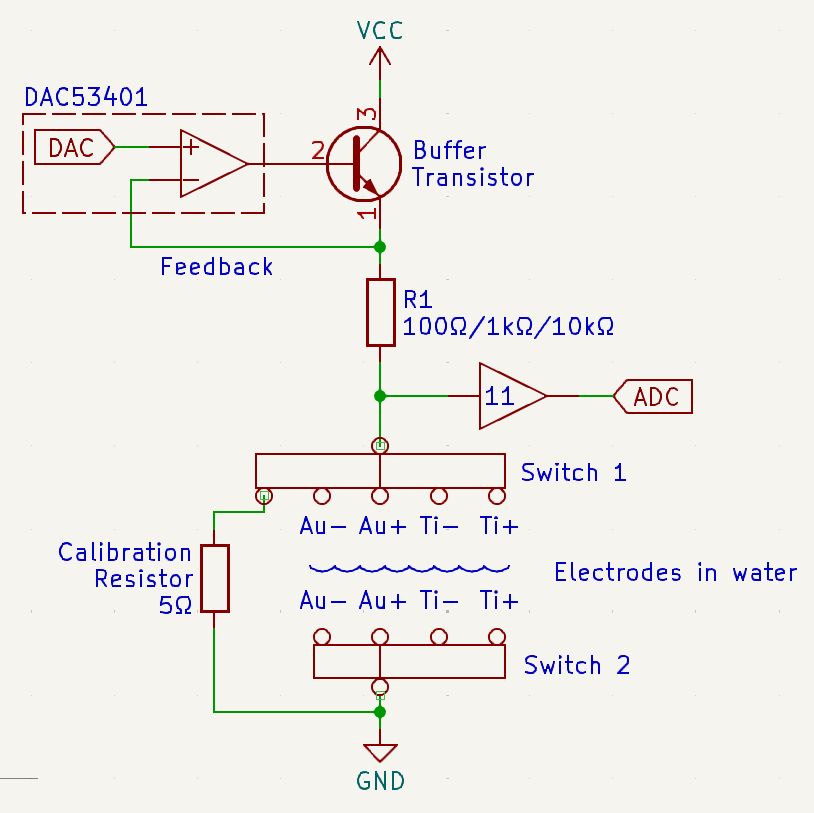
\includegraphics[width=0.5\textwidth]{Figures/CircuitOverview}
    \caption{A simplified representation of the resistance measuring circuit.}
    \label{fig:circuit-overview} %chktex 24
\end{figure}

\reffig{fig:circuit-overview} shows a simplified overview of the resistance measuring circuit that was used in this project.
The voltage driving the resistor divider was provided by a \gls{dac} such that the voltage could be varied and the resistance-voltage relationship could be determined for the titanium electrodes.
The resistance across the titanium electrodes remained uncertain and thus, in addition to the varied spacing and electrode length, alternative resistor values for $R_1$ were provided which could be selected using solder jumpers on the device.

The $R_1$ values were chosen to be $100\Omega$, $1k\Omega$ and $10k\Omega$ which would be used when the resistance between the probes is $1\Omega - 10\Omega$, $10\Omega - 100\Omega$ and $100\Omega - 1k\Omega$ respectively.
This would allow for a minimum resolution of $11\%$ of $V_{CC}$ for the voltage measurement by the \gls{adc} as shown by \refeqn{eqn:adc-resolution}.
\begin{equation}\label{eqn:adc-resolution}
    \lfrac{1\Omega}{1\Omega + 100\Omega} * 11 = 11\%
    \lfrac{10\Omega}{10\Omega + 100\Omega} * 11 = 100\%
\end{equation} 

Switch 1 allows $R_1$ to be connected to any of the four electrodes or a calibration resistor of $5\Omega$ and switch 2 allows for the other electrode to be connected to ground.
For example, switch 1 could be connected to Ti+ and switch 2 could be connected to Ti- to measure the resistance between the titanium electrodes.
This configuration also allows current to flow in both directions between electrodes which can prevent excessive build of chlorine gas or sodium electroplating on the electrodes by taking a resistance measurement in both directions in rapid succession.

In order to increase the measurement accuracy of the resistance, multiple high accuracy resistors were placed in series to attain the values of $R_1$ and the calibration resistor as this decreases the uncertainty of their resistance.
This decreases the total uncertainty $\delta_{R_{total}}$ by a factor of the number of parallel resistors $n$ compared to the individual resistor uncertainty $\delta_R$ as shown by \refeqn{eqn:parallel-resistor-total} to \refeqn{eqn:parallel-resistor-uncertainty}.
\begin{equation}[!h]\label{eqn:parallel-resistor-total}
    R_{total} = {\left[ \sum_{i=1}^{n} \lfrac{1}{R} \right]}^{-1} = {\left(\lfrac{n}{R}\right)}^{-1} = \lfrac{1}{n}\cdot R
\end{equation}
\begin{equation}[!h]\label{eqn:uncertainty-general-formula}
    \text{for a function}~f(x_1,x_2,\dots,x_n), \text{its uncertainty} ~\delta_f = \sqrt{\sum_{i=1}^{n} {\left( \lfrac{\partial f}{\partial x_i} \delta x_i \right)}^2}
\end{equation}
\begin{equation}[!h]\label{eqn:parallel-resistor-uncertainty}
    \therefore \delta_{R_{total}} = \sqrt{{\left( \lfrac{\partial R_{total}}{\partial R} \delta_R \right)}^2} = \sqrt{{\left( \lfrac{1}{n} \delta_R \right)}^2} = \lfrac{1}{n} \delta_R
\end{equation}
The resistances for $R_1$ were made from 3 parallel resistors with tolerance $\pm1\%$ giving a total uncertainty of $\pm0.\bar{3}\%$ and the calibration resistor was made from 4 parallel resistors with tolerance $\pm1\%$ giving a total uncertainty of $\pm0.25\%$.

\begin{figure}[!h]
    \centering
    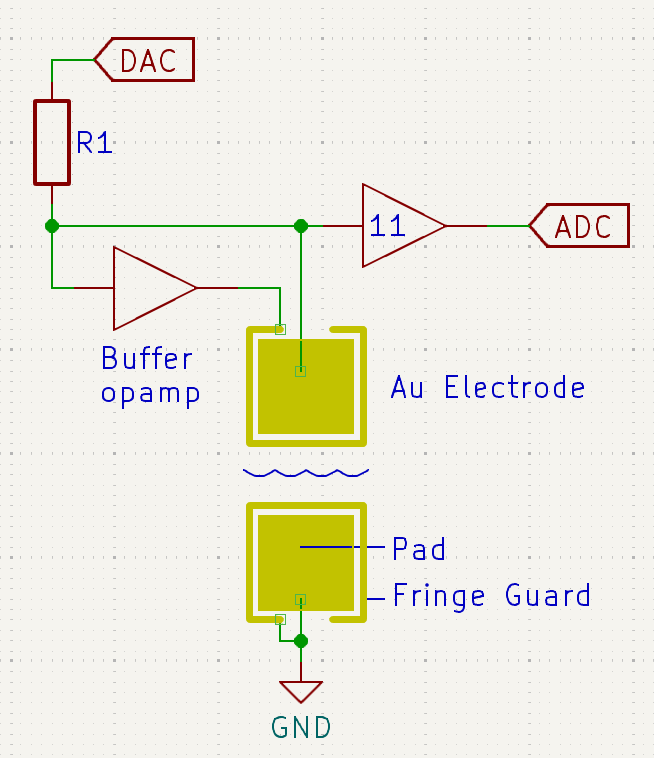
\includegraphics[width=0.5\textwidth]{Figures/AuElectrodeExample}
    \caption{A simplified representation of the resistance measurement circuit using the gold electrodes with the fringe guard.}
    \label{fig:au-measurement-circuit} %chktex 24
\end{figure}

\reffig{fig:au-measurement-circuit} shows an example switch configuration where the gold electrodes are used.
The buffer op-amp has unity gain and is used to repeat the voltage going to the pad of the top electrode to its fringe guard while the other pad and fringe guard are connected to ground.
In theory, this should allow for the fringing to be absorbed by the fringe guard and not affect the resistance measurement, however switches were added electrically connect or disconnect the fringe guard should it interfere with the resistance measurement.
The current flowing between the fringe guards was assumed to be less than that of the pads and thus there was no need to limit the current from the op-amp.

\subsection{Salinity Calculation and Display}

In order to measure the salinity of the sea ice, the probe needed to be lowered into the water and measure salinity at various depths.
There are two methods for capturing the salinity data: either to constantly record the salinity data as the device it lowered through the water column or to have the device take a measurement when instructed by a controller.
The former method creates logistical problems with waterproofing the device and retrieving data while the latter was a more user-friendly approach allowing researchers to control exactly which depths the salinity is measured at and was chosen for this project.

The controller consisted of a \gls{pcb} with input buttons and two output 7-segment displays to control and relay salinity information, and a RS485 communication port and a simple microcontroller.
The RS485 communication port was chosen as the communication protocol as RS485 has the longest range and a high noise resistance which is necessary for the device to be used in the ocean which has high \gls{emi}.
The microcontroller was arbitrarily chosen from the STM32F030 series as it was relatively cheap, and it did not need to perform any complex calculations.

With an external controller, a waterproofed probe could be lowered into the water and measure the water's salinity.
The chosen method of making a waterproof probe was to create a \gls{pcb} and coat it with a layer of epoxy resin to waterproof it as this was the most familiar and cost-efficient method available.
The probe \gls{pcb} was designed with the equipment necessary to measure the salinity including ports for the conductivity probes, the circuitry required to measure the resistance as shown in \reffig{fig:circuit-overview}, temperature and depth sensors which are discussed in \refsec{sec:temp-depth-measurement}, an RS485 communication port and a microcontroller.
The microcontroller that was chosen was from the STM32F401 series as STM microcontrollers as it had a \gls{fpu} which allowed for calculating salinity on the probe. 

\subsection{Temperature and Depth Measurement}\label{sec:temp-depth-measurement}

Depth sensors that a waterproof are too expensive for this projects budget.
However, there have been alternative approaches which use non-waterproof sensors that are isolated form the water using a flexible membrane that would allow the pressure to be transmitted to the sensor.
This project included a depth sensor with the aim to use this method to measure the depth of the probe in the water, however it also included a method for the user to manually input the depth of the probe in the water using the controller should this method fail.

The temperature sensor used in this project was an arbitrarily chosen, surface mount temperature sensor that had high accuracy and a wide temperature range.
The temperature sensor should be coated with a thin layer of epoxy resin to waterproof it as epoxy resin is a poor thermal conductor and thus a thinner layer would allow for a more accurate temperature measurement.
Lastly, as a convenient backup, the STM32F401 series of microcontroller contain a temperature sensor which is significantly less accurate with an accuracy of about $1\degree C$

\section{Device Coding}
ur mom

